\documentclass[10pt]{beamer}
\usepackage[utf8]{inputenc}
\usepackage[vietnamese]{babel}
\usepackage{booktabs}
\usepackage{tabularx}
\usepackage{graphicx}

\usetheme{Madrid}
\usecolortheme{default}
\setbeamertemplate{navigation symbols}{}

\title[Báo cáo tiến độ ĐATH]{Xây dựng hệ thống hỗ trợ chẩn đoán bệnh lý phổi từ ảnh X-quang lồng ngực sử dụng mô hình kiến trúc CNN/ViT và kỹ thuật giải thích mô hình Grad-CAM}
\author[Bảo, Huy]{
    \textbf{Giảng viên hướng dẫn:}\\
    \vspace{0.1cm}
    PGS. TS. Quản Thành Thơ\\
    \vspace{0.5cm}
    \textbf{Thành viên tham gia:}\\
    \vspace{0.1cm}
    Quách Gia Bảo\\
    Dương Quốc Huy\\
}
\date{Báo cáo tiến độ ngày 28/09/2026}

\begin{document}

\begin{frame}
    \titlepage
\end{frame}

\begin{frame}{Tổng quan đề tài}
    \textbf{Mục tiêu:} Xây dựng và đánh giá một hệ thống học sâu có khả năng nhận diện một số bất thường trên ảnh X-quang lồng ngực, tạo giải thích trực quan bằng Grad-CAM và đánh giá định lượng sự phù hợp giữa vùng giải thích của mô hình với chú thích (annotation) của bác sĩ.
    \vspace{0.3cm}

    \textbf{Các phần kỹ thuật cốt lõi:}
    \begin{itemize}
        \item Áp dụng Transfer Learning và Fine-tuning trên cả hai họ kiến trúc CNN (ResNet-50, DenseNet-121) và Vision Transformer (ViT-B/16) theo bài toán phân loại đa nhãn (Multi-label Classification).
        \item Cơ chế định vị và giải thích mô hình bằng Grad-CAM.
        \item Xây dựng hàm location-aware loss.
    \end{itemize}
\end{frame}

\begin{frame}{Câu hỏi nghiên cứu và giả thuyết}
    Đề tài được tổ chức xoay quanh hai câu hỏi nghiên cứu chính:

    \begin{block}{RQ1 -- Classification và localization}
        \textit{Does better classification imply better localization?}

        \medskip
        Mô hình có hiệu năng phân loại tốt hơn có đồng thời định vị vùng bất thường tốt hơn hay không?
    \end{block}

    \begin{block}{RQ2 -- Location-aware learning}
        Việc bổ sung location-aware loss có giúp Grad-CAM tập trung tốt hơn vào vùng bất thường được bác sĩ đánh dấu mà không làm suy giảm đáng kể hiệu năng phân loại hay không?
    \end{block}
\end{frame}

\begin{frame}{Outline}
    \begin{enumerate}
        \item Mô tả tập dữ liệu VinDr-CXR.
        \item Một số bài toán cần giải quyết.
        \item Các phương pháp giải quyết các bài toán đặt ra.
        \item Phương hướng tiếp theo.
    \end{enumerate}
\end{frame}

\begin{frame}{Outline}
    \centering
    \Large \textbf{1. Mô tả tập dữ liệu VinDr-CXR}
\end{frame}

\begin{frame}{Dữ liệu nghiên cứu: VinDr-CXR (1)}
    \begin{itemize}
        \item \textbf{Quy mô:} 18.000 ảnh X-quang lồng ngực (CXR) tư thế PA, gồm 15.000 ảnh huấn luyện và 3.000 ảnh kiểm thử.
        \item \textbf{Gán nhãn:} 17 bác sĩ chẩn đoán hình ảnh tham gia. Mỗi ảnh huấn luyện được đọc độc lập bởi 3 bác sĩ; tập kiểm thử sử dụng nhãn đồng thuận từ 5 bác sĩ.
        \item \textbf{Cấu trúc nhãn:} 28 nhãn, gồm 22 nhãn cục bộ (local labels) có khung bao (bounding box) và 6 nhãn toàn cục (global labels) phản ánh chẩn đoán ở mức ảnh.
        \item \textbf{Vai trò trong đề tài:} Hỗ trợ xây dựng quy trình chung cho phân loại (classification), đánh giá Grad-CAM và huấn luyện có thông tin vị trí (location-aware training).
    \end{itemize}
\end{frame}

\begin{frame}{Dữ liệu nghiên cứu: VinDr-CXR (2)}
    Mỗi một mẫu trong tập dữ liệu sẽ có các thông tin sau:
    \begin{itemize}
        \item Thông tin về nhãn (Disease): Thông tin của bệnh đã được gán nhãn trong ảnh được đề cập.
        \item Thông số Bounding Box: Là các hình chữ nhật với kích thước [($x_{min}$;$x_{max}$), ($y_{min}$;$y_{max}$)]. Đại diện cho các vùng bất thường được thể hiện trên ảnh XRay.
        \item Định danh của bác sĩ đánh giá: Theo các giá trị ẩn danh từ $R_1$ đến $R_{17}$.
    \end{itemize}
    \vspace{1em}
    Trong đó, mỗi ảnh được đánh giá bởi 3 bác sĩ, và mỗi đánh giá có thể có nhiều nhãn khác nhau. Đồng thời, có một vài nhãn không có thông số Bounding Box.
\end{frame}

\begin{frame}{Preprocessing}
    Tập dữ liệu ban đầu là dữ liệu ảnh DICOM, với dung lượng lớn cùng với thông tin Bounding Box chưa được chuẩn hóa. Do đó, nhóm xử lí theo các bước:
    \begin{itemize}
        \item Đọc và chuyển đổi ảnh X-quang từ định dạng DICOM.
        \item Resize toàn bộ ảnh về kích thước thống nhất.
        \item Điều chỉnh tọa độ bounding box tương ứng với kích thước ảnh sau khi resize.
        \item Dữ liệu sau tiền xử lý được sử dụng cho EDA và làm đầu vào cho pipeline huấn luyện.
    \end{itemize}
    Các kiến trúc backbone dự kiến sử dụng (ResNet-50, DenseNet-121, Vision Transformer ViT-B/16) đều là các mô hình được huấn luyện trên tập dữ liệu ImageNet với kích thước chuẩn mặc định là $224 \times 224$, do đó, kích thước ảnh đầu vào sau khi tiền xử lí sẽ là $224 \times 224$, đồng thời cũng là kích thước của Ma trận nhị phân $G_c$.   
\end{frame}


\begin{frame}{Phân phối lớp và mất cân bằng nhãn}
    \begin{center}
        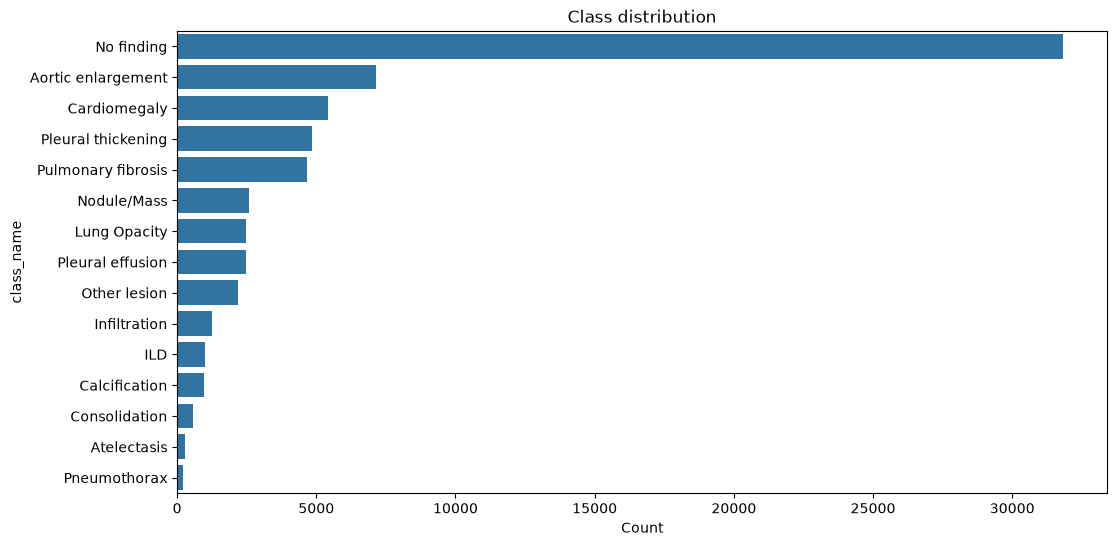
\includegraphics[width=0.94\textwidth,height=0.57\textheight,keepaspectratio]{../figures/28-9-2026/class-distr.png}
    \end{center}
    \vspace{-0.15cm}
    \small
    \begin{itemize}
        \item Nhãn \textit{No finding} chiếm ưu thế rõ rệt, trong khi nhiều lớp bệnh lý có số lượng mẫu rất thấp.
        \item Phân phối dạng long-tail có thể khiến mô hình thiên lệch về lớp phổ biến và giảm khả năng nhận diện các bất thường hiếm.
        \item Ảnh hưởng tới hàm mất mát của Classification task.
    \end{itemize}
\end{frame}


\begin{frame}{Local labels vs. Global labels (1)}
    \begin{columns}[T]
        \begin{column}{0.48\textwidth}
            \textbf{Local labels}
            \begin{itemize}
                \item Có bounding box xác định vị trí bất thường.
                \item Phục vụ classification, localization và đánh giá Grad-CAM.
                \item Gồm 22 lớp trong VinDr-CXR.
            \end{itemize}
        \end{column}
        \begin{column}{0.48\textwidth}
            \textbf{Global labels}
            \begin{itemize}
                \item Chỉ có nhãn chẩn đoán ở mức toàn ảnh.
                \item Không cung cấp annotation vị trí trực tiếp.
                \item Gồm 6 lớp trong VinDr-CXR.
            \end{itemize}
        \end{column}
    \end{columns}
    \vspace{1em}
    Theo nội dung của các câu hỏi nghiên cứu (RQ1, RQ2) mà đề tài hướng tới, cần tập trung những mẫu dữ liệu có Bounding Box để so sánh giữa các mô hình trên location-aware learning.
\end{frame}

\begin{frame}{Local labels vs. Global labels (2)}
    \begin{center}
        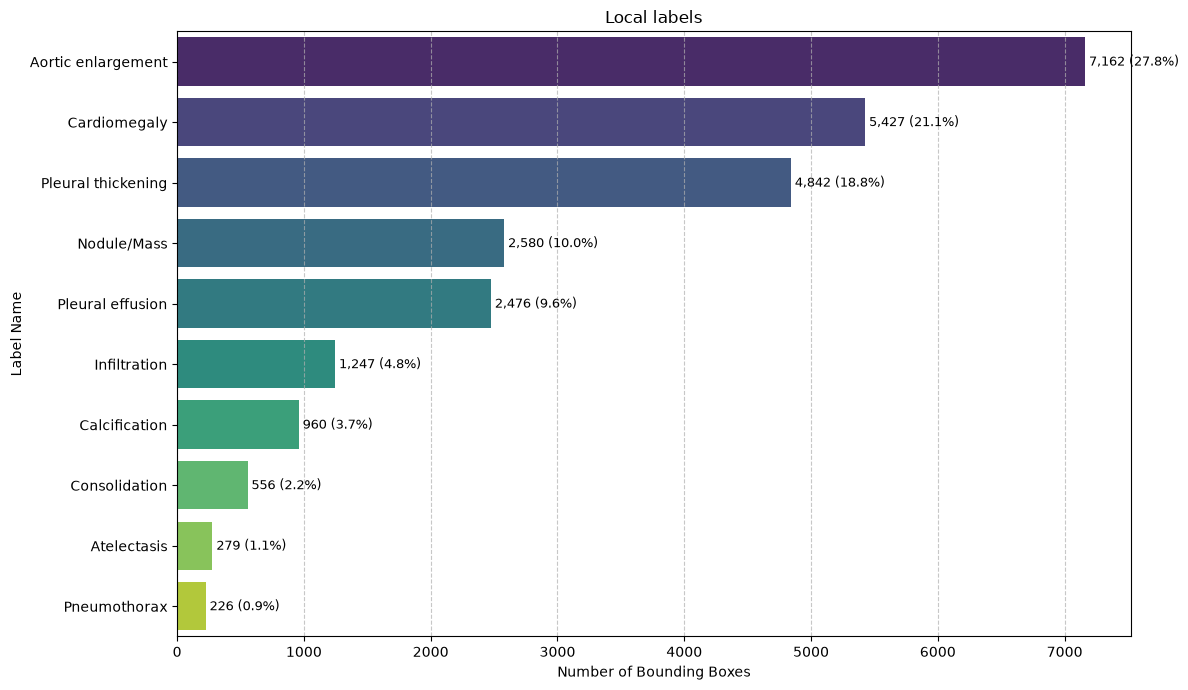
\includegraphics[width=0.96\textwidth,height=0.78\textheight,keepaspectratio]{../figures/28-9-2026/local-label-distr.png}
    \end{center}
\end{frame}

\begin{frame}{Outline}
    \centering
    \Large \textbf{2. Một số bài toán cần giải quyết}
\end{frame}

\begin{frame}{EDA và các vấn đề cần giải quyết}\small
    Từ đặc điểm của VinDr-CXR, nhóm xác định năm bài toán cần giải quyết:
    \begin{enumerate}
        \item \textbf{Localization classes:} Chỉ các mẫu có bounding box mới tham gia $L_{loc}$ và hỗ trợ cho các giả thiết nghiên cứu của đề tài; các mẫu không có bounding box chỉ sử dụng cho task classification.
        \item \textbf{Data agreement:} Do mỗi mẫu dữ liệu do 3 bác sĩ khác nhau đánh giá, cần đánh giá và thống nhất phương pháp để hợp nhất: Bounding Box Annotation và Classification.
        \item \textbf{Multi-label classification:} Phân tích số bệnh trên mỗi ảnh và quan hệ giữa các nhãn (Các bệnh có đi chung với nhau không?), đồng thời giải quyết tình trạng mất cân bằng mẫu của tập dữ liệu.
        \item \textbf{Phân phối diện tích bounding box:} So sánh diện tích tổn thương với diện tích toàn cục của ảnh để đánh giá độ khó của Grad-CAM và location-aware loss theo từng lớp.
        \item \textbf{Tạo ground-truth mask:} Xây dựng quy tắc consensus (hay fusion) từ annotation của ba bác sĩ khác nhau để tạo binary mask $G_c$ kích thước $224 \times 224$.
    \end{enumerate}

    \vspace{0.1cm}
    \textbf{Đầu ra:} Quy tắc hợp nhất annotation và thiết kế loss cho các thí nghiệm tiếp theo.
\end{frame}

\begin{frame}{Outline}
    \centering
    \Large \textbf{3. Các phương pháp giải quyết bài toán}
\end{frame}

\begin{frame}{Bài toán Data Agreement (1)}
    Mỗi mẫu dữ liệu do 3 bác sĩ khác nhau đánh giá, trong đó, các giá trị quan trọng cần thiết kế là sự đồng thuận giữa các nhãn bệnh và các bounding box. Do đó, ta sẽ có 2 bài toán nhỏ hơn.
    \begin{itemize}
        \item Class Agreement: Đâu là các nhãn đại diện cho các bất thường trên ảnh trên 3 tập nhãn đánh giá khác nhau?
        \item Bounding Box Agreement: Với những nhãn được xác định, nếu 2 bác sĩ xác định 2 Bounding box có giá trị khác nhau xét về mặt số liệu, thì đâu mới là vùng bất thường dựa trên 2 mẫu dữ liệu đó?
    \end{itemize}
\end{frame}

\begin{frame}{Bài toán Data Agreement (2)}
    Để xác định Consensus rule cho Class Agreement trong bài toán hiện tại, chúng ta có các phương pháp sau:
    \begin{itemize}
        \item \textbf{Majority Vote}: Từ các kết quả của các bác sĩ, chọn ra các nhãn có độ đồng thuận từ 2 trở lên.
        \item Unanimous: Chỉ bao gồm những nhãn có độ đồng thuận tối đa.
        \item Any Vote: Các nhãn có độ đồng thuận từ 1 trở lên.
    \end{itemize}
    \begin{center}
        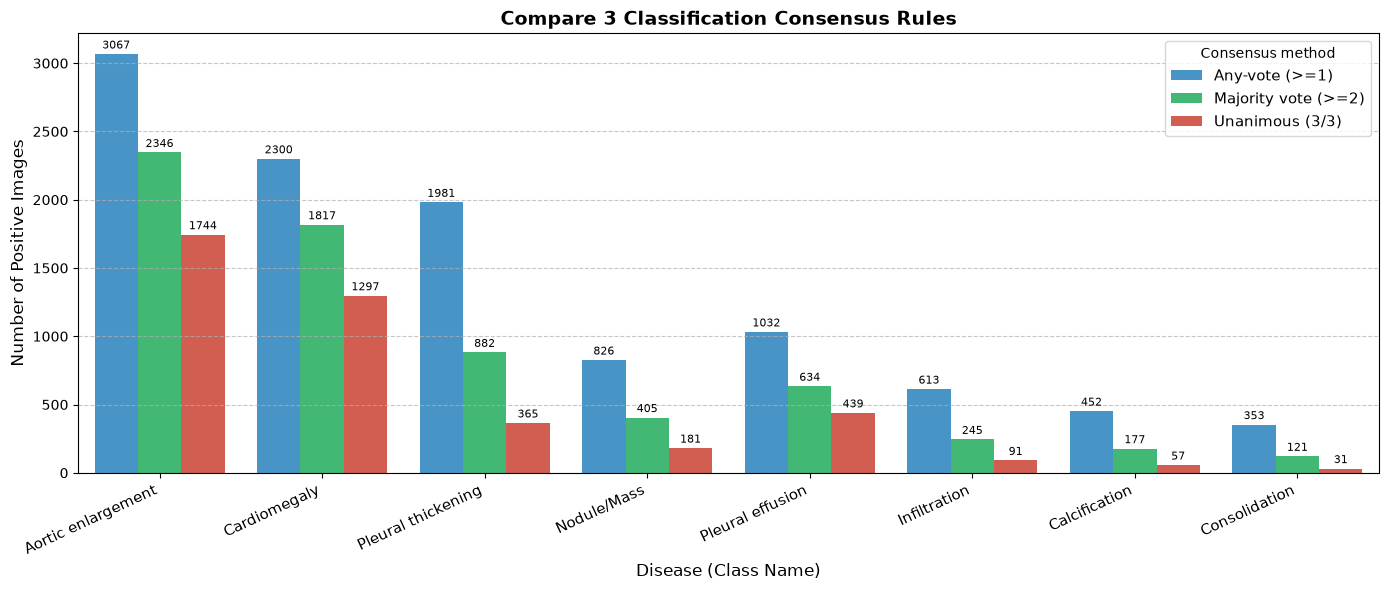
\includegraphics[width=0.96\textwidth,height=0.78\textheight,keepaspectratio]{../figures/28-9-2026/class-agreement-distr.png}
    \end{center}
\end{frame}

\begin{frame}{Bài toán Data Agreement (3)}
    Để tính được hàm mất mát định vị Inside-Box Energy Loss ($L_{loc}$
    $$L_{loc} = 1 - \frac{\sum (A_c \odot G_c)}{\sum A_c + \epsilon}$$
    Ta bắt buộc phải hợp nhất các annotation riêng rẽ này thành một nhãn vị trí chuẩn ($G_c$).
    \begin{itemize}
        \item IoU clustering with Union Box: trên mỗi Bounding Box khác nhau trên cùng 1 ảnh, xác định giá trị IoU, sau đó gom cụm lại trên 1 threshold được xác định trước.
        \item Pixel-Level Consensus Masking: Mỗi bác sĩ $k \in \{1, 2, 3\}$, vẽ các bounding box của họ lên một ma trận nhị phân $M_k \in \{0, 1\}^{224 \times 224}$. 
        $$M_{sum}(x, y) = \sum_{k=1}^K M_k(x, y)$$
        Sau đó, dùng Majority-voted mask để xác định ground truth $G_c$: $G_c(x, y) = 1 \iff M_{sum}(x, y) \ge 2$
    \end{itemize}
\end{frame}

\begin{frame}{Bài toán Data Agreement (4)}
    \begin{center}
        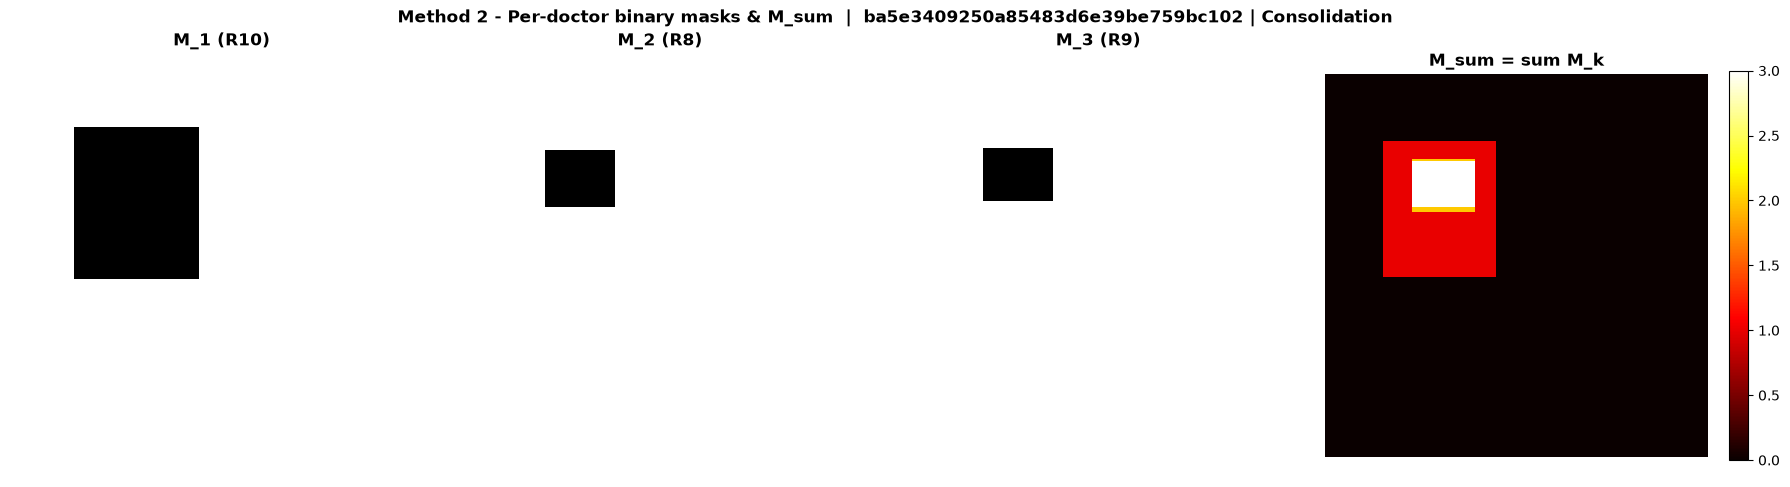
\includegraphics[width=0.98\textwidth,height=0.70\textheight,keepaspectratio]{../figures/28-9-2026/per-dr-masks-fig-2.png}
    \end{center}
    \small
    Mỗi bounding box được chuyển thành binary mask $M_k$. Tổng $M_{sum}$ biểu diễn số bác sĩ cùng đánh dấu tại từng pixel và là cơ sở để xây dựng consensus mask.
\end{frame}

\begin{frame}{Bài toán Data Agreement (5)}
    \begin{center}
        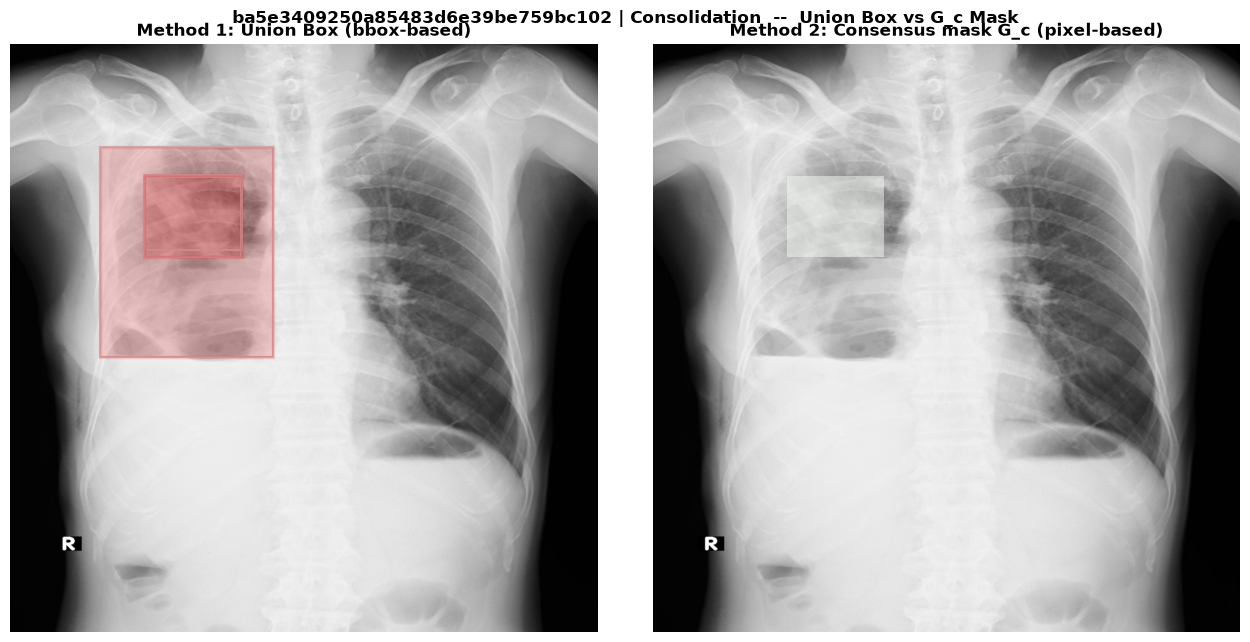
\includegraphics[width=0.98\textwidth,height=0.70\textheight,keepaspectratio]{../figures/28-9-2026/ex-consensus-fig-2.png}
    \end{center}
    \small
    So sánh hai cách hợp nhất annotation: Union Box giữ toàn bộ vùng bao phủ, trong khi pixel-level consensus chỉ giữ vùng đạt ngưỡng đồng thuận giữa các bác sĩ.
\end{frame}

\begin{frame}{Bài toán Class Imbalance (1)}
    Trong bài toán phân loại đa nhãn trên ảnh CXR, số mẫu âm tính của mỗi lớp thường lớn hơn nhiều so với số mẫu dương tính. Ngay cả với lớp phổ biến như \textit{Aortic enlargement}, phần lớn ảnh vẫn không mang nhãn này.

    \vspace{0.15cm}
    Hàm Binary Cross-Entropy (BCE) thông thường được xác định bởi:
    \[
        L_{\mathrm{BCE}}
        = -\frac{1}{C}\sum_{c=1}^{C}
        \left[y_c\log p_c + (1-y_c)\log(1-p_c)\right].
    \]

    \begin{itemize}
        \item Khi $N_{neg}^{(c)} / N_{pos}^{(c)} \gg 1$, thành phần từ các mẫu âm tính chi phối quá trình tối ưu.
        \item Mô hình có xu hướng ưu tiên dự đoán âm tính, làm giảm khả năng phát hiện các bệnh hiếm.
        \item Vì vậy, $L_{cls}$ cần được điều chỉnh để tăng mức phạt đối với các mẫu dương tính bị bỏ sót.
    \end{itemize}
\end{frame}

\begin{frame}{Bài toán Class Imbalance (2)}
    \textbf{Weighted BCE:} Gán trọng số riêng cho mẫu dương tính của từng lớp:
    \[
        L_{\mathrm{wBCE}}
        = -\frac{1}{C}\sum_{c=1}^{C}
        \left[w_{pos}^{(c)}y_c\log p_c + (1-y_c)\log(1-p_c)\right],
        \qquad
        w_{pos}^{(c)} = \frac{N_{neg}^{(c)}}{N_{pos}^{(c)}}.
    \]

    \textbf{Focal Loss:} Giảm ảnh hưởng của các mẫu dễ và tập trung vào các mẫu khó:
    \[
        L_{\mathrm{Focal}}
        = -\frac{1}{C}\sum_{c=1}^{C}
        \alpha_c(1-p_{t,c})^{\gamma}\log p_{t,c}.
    \]

    \textbf{Asymmetric Loss:} Sử dụng hệ số tập trung khác nhau cho mẫu dương và âm; có thể bỏ qua các mẫu âm dễ bằng ngưỡng dịch $m$:
    \[
        L_{\mathrm{ASL}}
        = -\frac{1}{C}\sum_{c=1}^{C}
        \left[y_c(1-p_c)^{\gamma_+}\log p_c
        +(1-y_c)p_{m,c}^{\gamma_-}\log(1-p_{m,c})\right].
    \]
\end{frame}

\begin{frame}{Outline}
    \centering
    \Large \textbf{4. Phương hướng tiếp theo}
\end{frame}

\begin{frame}{Một số công việc tiếp theo}
    \begin{itemize}
        \item Hiện thực các backbone theo pipeline đề xuất, gồm ResNet-50, DenseNet-121 và Vision Transformer (ViT).
        \item Hiện thực các metric phục vụ đánh giá kết quả thí nghiệm về classification và localization.
        \item Nghiên cứu, lựa chọn và hiện thực các hàm mất mát phù hợp với bài toán phân loại đa nhãn và location-aware learning.
    \end{itemize}
\end{frame}


\end{document}